% Chapter 4 as a single file -- merged 2026-09-20 from chapter_04_setup.tex and the four section
% files it input (_sec41_collection, _sec42_system_overview, _sec43_scoring_calibration,
% _sec44_judge), which are kept as *.preMerge.bak.tex and no longer input. Text unchanged by the
% merge; edit THIS file from now on (manifest §4d, 2026-09-20).
\chapter{Experimental Setup}\label{ch:setup}

% ---------------------------------------------------------------------------
% SHARED ONLY. Admission test (manifest §8): would RQ2 need this even if RQ1 did
% not exist, and RQ1 even if RQ2 did not? Four things pass (revised 2026-09-20): the
% material, the system, and the two preconditions P1 and P2. The notation section (was
% §4.5) was removed 2026-09-20 -- coined terms are defined at first use in the RQ chapter
% that needs them (manifest §15 O-14); it may return if required. Tie-breaker:
% what depends on an RQ's own object stays with that RQ; Chapter 6 cites Chapter 5
% backwards. Everything that fails the test lives inside the RQ chapter that uses it.
% Definitions of the collection, its tasks, its relevance levels and its pooling
% belong to §3.1 -- this chapter states what was taken from them.
% Chapter opener written 2026-09-19.
% ---------------------------------------------------------------------------

The retrieval and generation chapters each answer one research
question, and each is meant to be read as a complete argument of its own. That
works only if what the two share is fixed before either begins, and fixing it is
what this chapter is for. Chapter~\ref{ch:background} defined what the
collection, the formula representations, the retrieval and fusion methods and the
evaluation measures are; this chapter states what this thesis did with them that
both questions depend on. Whatever only one question uses is described in that
question's own chapter: how the indices are built and combined belongs to
retrieval, and how answers are generated and scored belongs to generation.

Section~\ref{sec:met-collection} fixes the material --- the topics, the relevance
judgments taken from ARQMath, and the corpus as the system reads it --- and
Section~\ref{sec:met-system-overview} describes the system end to end, marking
which part of it each question studies. Sections~\ref{sec:met-calibration}
and~\ref{sec:met-judge-validation} establish the two
preconditions of Section~\ref{sec:intro-rqs}. The first is that the scoring code
is correct. The second is that a language model can judge relevance well enough to
rank systems the way the human assessors do. Every retrieval score in this thesis
rests on both, and the generation chapter reads retrieval quality through
those same scores, which is why neither precondition belongs to retrieval alone.

% --- §4.1 Topics, qrels and preprocessing ----------------------------------
% Rewritten 2026-09-19. The 78-topic Task 1 judgments only; Task 2's judgments are
% Chapter 5's; the formula representation files moved to §5.2.1.
% Chapter 4 section 4.1: topics, qrels and preprocessing.
% Rewritten 2026-09-19 (manifest §8 row 4.1). Shared material only: the Task 1 topics and
% judgments both RQs are evaluated on, and the corpus as the system reads it.
% Decided 2026-09-19: Task 2's topics and judgments are Chapter 5's; the formula representation
% files moved to §5.2.1; no qrels file is named other than the 78-topic one, and neither the
% 100 released topics nor any 87-topic set is mentioned.

\section{Topics, qrels and preprocessing}\label{sec:met-collection}

Both research questions are answered on the same answer-retrieval topics and scored against
judgments from the same collection, so which topics and which judgments are used
fixes what the numbers in the two chapters that follow mean.
Section~\ref{sec:bg-arqmath} described the collection, its tasks and how its
judgments were pooled. This section states which of its topics and judgments this
thesis uses, and for what, and how the corpus is turned into the files the system
reads.

Every retrieval and generation experiment on answer retrieval in this thesis is evaluated on
the 78 topics of the ARQMath-3 test collection (Section~\ref{sec:bg-arqmath});
Table~\ref{tab:met-qrels} summarises the organisers' relevance judgments for them.
Formula search keeps its own topics and judgments, and the retrieval chapter describes
them where it uses them. One further set of judgments is used, and this thesis
produces it rather than taking it from ARQMath: the relevance judge's labels for
the answers the retrieval systems return. Section~\ref{sec:met-evaluation-protocol}
describes how they are pooled, once the judge itself has been introduced.

\begin{table}[t]
\centering
\begin{tabular}{rrrrrr}
\toprule
Topics & High & Medium & Low & Not relevant & Total \\
\midrule
78 & 867 & 2{,}076 & 4{,}921 & 26{,}983 & 34{,}847 \\
\bottomrule
\end{tabular}
\caption[The ARQMath-3 relevance judgments]{The ARQMath-3 answer-retrieval relevance judgments: the number of judged (topic,
answer post) pairs at each relevance level, over the 78 topics of the evaluated
test collection.}
\label{tab:met-qrels}
\end{table}

The judgments of the two earlier editions, ARQMath-1 and ARQMath-2, enter the
thesis in one place only: together with those of ARQMath-3, they are what the
relevance judge is validated against. In all three editions at least three quarters
of the judged pairs are Not relevant, and High is the rarest label; over the 78
topics, 26{,}983 of the 34{,}847 pairs are Not relevant and 867 are High.
Relevance is rare, and Section~\ref{sec:met-judge-validation} returns to what that
rarity does to the judge's agreement with the assessors.

The collection is distributed as a single XML file, \texttt{Posts.V1.3.xml}, in
which each post is one \texttt{row} element holding the post as HTML, every formula
marked up in place and tagged with its collection identifier. Each post in the
collection is marked as either a question or an answer (the \texttt{PostTypeId}
attribute, 1 or 2), and the parse writes the two to separate JSON Lines files:
1{,}445{,}495 answers and 1{,}020{,}585 questions. Parsing strips the markup and
leaves the \LaTeX{} of each formula in place in the plain text, and additionally
collects those formulas into a separate per-post list, so that one pass yields both
the text that sparse and dense retrieval search and the formula list that formula
retrieval needs. An answer record keeps its identifier, the identifier of the
question it answers, its community score, the body text and the formula list. The
community score is retained because the reference used for generation evaluation
ranks candidate answers by it.

The topics are parsed from the ARQMath-3 Task~1 topic file into a third JSON Lines
file, each record keeping the topic's title and question body with their formulas
handled as in the posts.

These are the inputs both research questions share: the answer posts the system
searches, the topics it answers, and the judgments it is scored against. How the
system turns a topic into a ranked list of answer posts, and how the top of that
list is handed to the generator as context --- where retrieval ends and generation
begins --- is what Section~\ref{sec:met-system-overview} lays out.

% --- §4.2 System overview -------------------------------------------------
% Figure (fig:met-system-overview) and prose written 2026-09-19.
% Chapter 4 section 4.2: system overview.
% Prose written 2026-09-19 (manifest §8 row 4.2), reviewed in the chat before it was written here.
%   Walks the two phases (offline build, online answer) against the figure, places the hand-over
%   at the ranked list, and says what each RQ varies and holds fixed: RQ1 never generates; RQ2
%   varies the context and the generator's size (RQ2.3 / H2.4, 2026-09-19) and holds fixed the
%   ranked lists, the prompt and the decoding. Ends by handing over to §4.3.
%   Uses none of §4.5's vocabulary (channel, configuration, run, condition, judge pool) and states
%   no outcome of any hypothesis.
% Figure: the §12 pipeline as one full-page figure, annotated with the RQ boundary -- upper band
% RQ1 (L0-L4, plus Task 2 and retrieval measurement), lower band RQ2 (L5 and generation
% measurement). Grey = shared by both RQs (Chapter 4). Simplified by Abram 2026-09-19; restyled
% the same day. Core TikZ only: no \usetikzlibrary is needed. Names no checkpoint -- those
% belong to §5.2 and §6.2.

\section{System overview}\label{sec:met-system-overview}

The retrieval and generation chapters study two parts of one system, and
each reads as a complete argument only if it is clear where its part begins and ends.
This section describes the system end to end, in Figure~\ref{fig:met-system-overview},
and marks the point at which one research question hands over to the other. The
hand-over fixes what each chapter varies and what it holds
still.

The system works in two phases. The first happens once, offline, before any topic is
seen, and builds the indices. Each of the answer posts of
Section~\ref{sec:met-collection} is indexed three ways: its text in a sparse index scored
by BM25, the same text as a single bi-encoder vector in a dense index, and its formulas
in a formula index. There are three formula indices rather than one, one for each of the
tree representations of Section~\ref{sec:bg-formula-representations}, because each
representation keeps different information about the same formula, and whether that
difference matters for answer retrieval is a question the retrieval chapter takes
up. The same formula embeddings are also indexed over every formula in the collection,
to be queried with a single formula. That is formula search, and it
lets the formula index be examined on the task its representations were designed for
before it is asked to retrieve answers.

The second phase happens once per topic. The topic's text is sent to the sparse and
dense indices and its formulas to the formula indices, so a single topic yields five
ranked lists of answer posts. The reciprocal rank fusion of
Section~\ref{sec:bg-rank-fusion} merges two or more of them into one, or a single list
is used on its own; either way the topic ends with one ranked list, and retrieval ends
there. Generation starts from the head of that list. Its top $k$ posts become the
context of Section~\ref{sec:bg-generation-metrics}, and the generator, a language model,
answers the topic's question given that context and one fixed prompt.

The hand-over falls at the ranked list, and it divides the figure into its two bands.
RQ1 studies everything above it --- which indices are searched, which formula
representation is used, how the lists are fused --- and scores the ranked list itself.
The generator plays no part in that: every score in the retrieval chapter is
computed from what retrieval returns, before any answer has been generated, so nothing
on the generation side can change it.
RQ2 studies everything below the hand-over and varies two things. The first is the
context: where its posts come from, or whether there is a context at all. The second is
the size of the generator, since RQ2 also asks whether what retrieval adds depends on
how much the generator already knows. The retrieval side is held fixed throughout. Each
ranked list reaches the generator exactly as the retrieval chapter produced it,
with no index rebuilt and no list re-ranked, and the prompt and decoding settings are the
same for every answer. The generator changes only between comparisons, never within one,
so that two answers to the same topic from the same generator differ only in what they
were given to read.

The right-hand column of the figure shows what each question is scored with. A ranked
list is scored with the prime measures of Section~\ref{sec:bg-retrieval-metrics},
against relevance labels from the assessors and from a relevance judge; an answer is
scored with the RAGAS measures of Section~\ref{sec:bg-generation-metrics}, faithfulness
against its context and factual correctness against a reference.
The generation chapter uses the retrieval chapter's scores as
well: to ask whether better retrieval produces better answers, it sets each ranked list's
score beside the faithfulness and factual correctness of the answers generated from it.
Both questions therefore rest on the same retrieval scores.
That is why the parts shaded grey --- the
material of Section~\ref{sec:met-collection} and the two instruments behind those scores
--- are described in this chapter rather than in either of the next two. Whether the
first of them, the scoring code, is correct is the question
Section~\ref{sec:met-calibration} settles.

\begin{figure}[p]
\centering
% Bands and card stacks sit on layers beneath the cards, so that they can be sized from
% the cards drawn on top of them.
\pgfdeclarelayer{sysbg}
\pgfdeclarelayer{sysstack}
\pgfsetlayers{sysbg,sysstack,main}
\definecolor{rqoneband}{RGB}{234,241,250}
\definecolor{rqoneink}{RGB}{38,78,138}
\definecolor{rqtwoband}{RGB}{251,241,228}
\definecolor{rqtwoink}{RGB}{158,82,18}
\definecolor{sharedfill}{RGB}{233,233,233}
% \figtag prints the small grey section pointers; \renewcommand{\figtag}[1]{} hides them all.
\newcommand{\figtag}[1]{\hspace{0pt plus 1filll}{\color{black!50}\sffamily\tiny #1}}
\newcommand{\figsub}[1]{{\color{black!72}#1}}
\ifdefined\figlabelw\else\newlength{\figlabelw}\newlength{\figya}\newlength{\figyb}\fi
\settowidth{\figlabelw}{\footnotesize\textbf{RQ2}\enspace Generation $\cdot$
  Chapter~\ref*{ch:generation}}% length of the lower band's rotated label
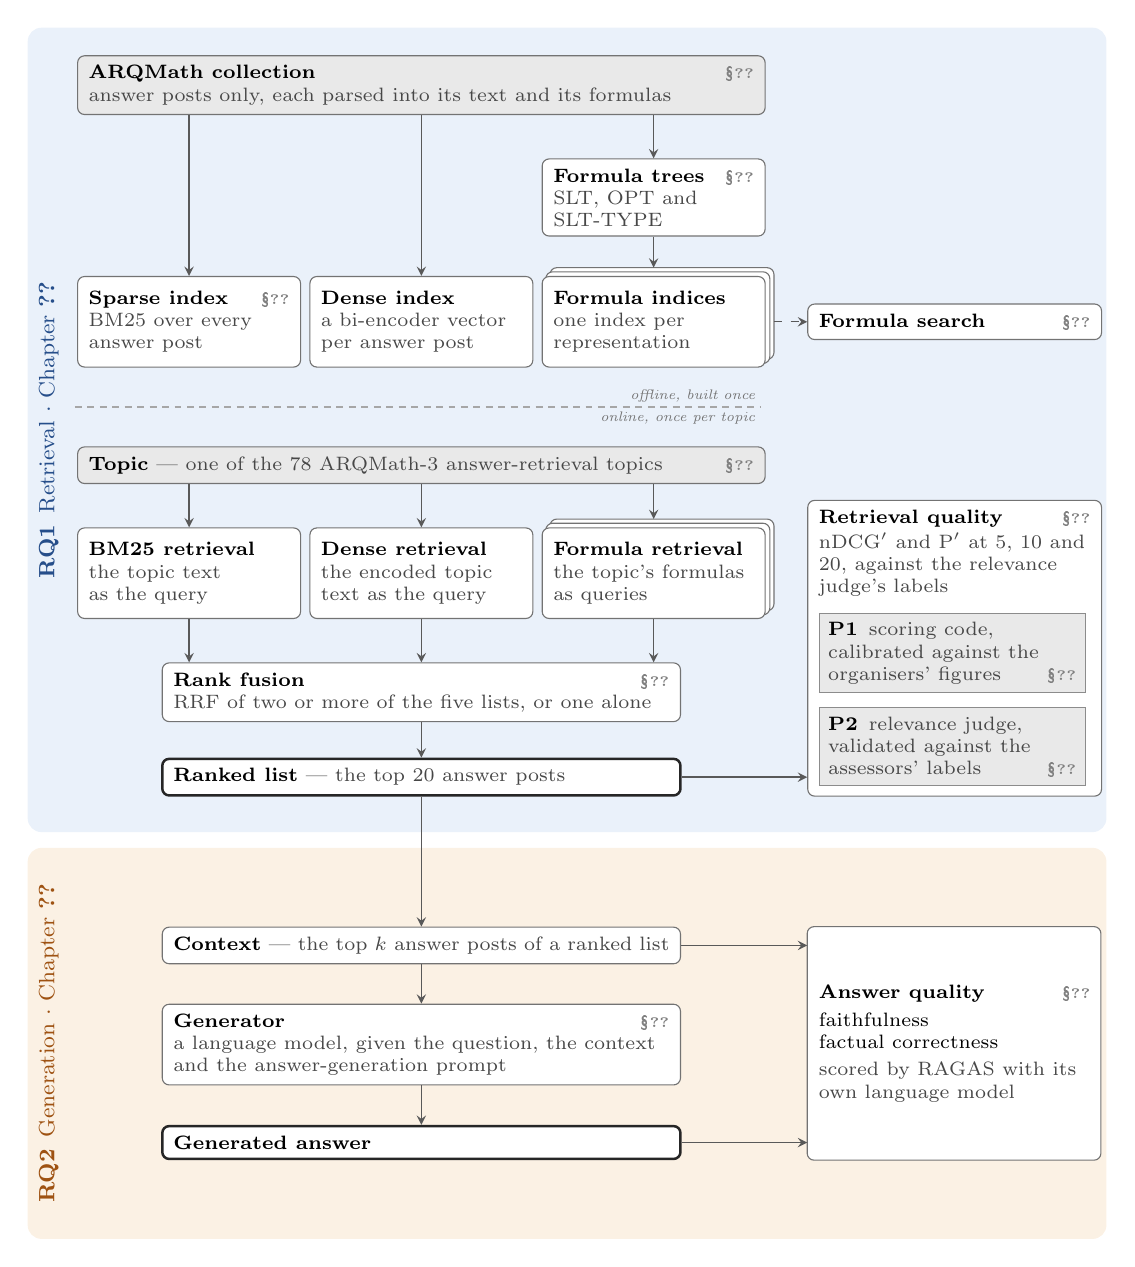
\begin{tikzpicture}[
    >=stealth,
    font=\scriptsize,
    card/.style={draw=black!55, rounded corners=2.5pt, fill=white, align=flush left,
                 inner xsep=4pt, inner ysep=3.5pt, line width=0.4pt,
                 execute at begin node={\hyphenpenalty=10000\exhyphenpenalty=10000}},
    lane/.style={card, text width=2.55cm, minimum height=1.15cm},
    wide/.style={card, text width=8.45cm},
    mid/.style={card, text width=6.3cm},
    side/.style={card, text width=3.45cm},
    shared/.style={fill=sharedfill},
    key/.style={draw=black!85, line width=0.9pt},
    flow/.style={->, draw=black!65, line width=0.5pt},
  ]
  \hypersetup{linkcolor=black!50}% the section tags' numbers in the tags' grey

  % ============================================================ RQ1 -- offline
  \node[wide, shared, anchor=north] (coll) at (5.0,-0.35)
    {\textbf{ARQMath collection}\figtag{\S\ref{sec:met-collection}}\\
     \figsub{answer posts only, each parsed into its text and its formulas}};

  \node[lane, minimum height=0.95cm, below=5.5mm] (trees) at (coll.south -| 7.95,0)
    {\textbf{Formula trees}\figtag{\S\ref{sec:met-formula-indexing}}\\
     \figsub{SLT, OPT and \mbox{SLT-TYPE}}};
  \node[lane, below=5mm] (ixF) at (trees.south)
    {\textbf{Formula indices}\\ \figsub{one index per representation}};
  \node[lane, anchor=north] (ixD) at (ixF.north -| 5.0,0)
    {\textbf{Dense index}\\ \figsub{a bi-encoder vector per answer post}};
  \node[lane, anchor=north] (ixS) at (ixF.north -| 2.05,0)
    {\textbf{Sparse index}\figtag{\S\ref{sec:met-retrieval-configs}}\\
     \figsub{BM25 over every answer post}};

  \draw[flow] (coll.south -| ixS.north)   -- (ixS.north);
  \draw[flow] (coll.south -| ixD.north)   -- (ixD.north);
  \draw[flow] (coll.south -| trees.north) -- (trees.north);
  \draw[flow] (trees) -- ([yshift=3pt]ixF.north);

  % Task 2: the formula stack on its own
  \node[side, anchor=west] (t2) at (ixF.east -| 9.9,0)
    {\textbf{Formula search}\figtag{\S\ref{sec:guard-task2}}};
  \draw[flow, dashed] ([xshift=3pt]ixF.east) -- (t2.west);

  % ============================================================ phase line
  \coordinate (ph) at ([yshift=-5mm]ixF.south);
  \draw[black!35, dash pattern=on 2.5pt off 2pt, line width=0.4pt]
    (ph -| 0.6,0) -- (ph -| 9.3,0);
  \node[font=\tiny\itshape, text=black!55, anchor=south east, inner sep=1.5pt]
    at (ph -| 9.3,0) {offline, built once};
  \node[font=\tiny\itshape, text=black!55, anchor=north east, inner sep=1.5pt]
    at (ph -| 9.3,0) {online, once per topic};

  % ============================================================ RQ1 -- online
  \node[wide, shared, anchor=north] (topic) at ([yshift=-5mm]ph -| 5.0,0)
    {\textbf{Topic} \figsub{--- one of the 78 ARQMath-3 answer-retrieval topics}%
     \figtag{\S\ref{sec:met-collection}}};

  \node[lane, anchor=north] (sS) at ([yshift=-5.5mm]topic.south -| 2.05,0)
    {\textbf{BM25 retrieval}\\ \figsub{the topic text\\ as the query}};
  \node[lane, anchor=north] (sD) at ([yshift=-5.5mm]topic.south -| 5.0,0)
    {\textbf{Dense retrieval}\\ \figsub{the encoded topic text as the query}};
  \node[lane, anchor=north] (sF) at ([yshift=-5.5mm]topic.south -| 7.95,0)
    {\textbf{Formula retrieval}\\ \figsub{the topic's formulas as queries}};

  \draw[flow] (topic.south -| sS.north) -- (sS.north);
  \draw[flow] (topic.south -| sD.north) -- (sD.north);
  \draw[flow] (topic.south -| sF.north) -- ([yshift=3pt]sF.north);

  \node[mid, anchor=north] (fus) at ([yshift=-5.5mm]sS.south -| 5.0,0)
    {\textbf{Rank fusion}\figtag{\S\ref{sec:met-retrieval-configs}}\\
     \figsub{RRF of two or more of the five lists, or one alone}};
  \draw[flow] (sS.south) -- (sS.south |- fus.north);
  \draw[flow] (sD.south) -- (sD.south |- fus.north);
  \draw[flow] (sF.south) -- (sF.south |- fus.north);

  \node[mid, key, below=4.5mm] (rl) at (fus.south)
    {\textbf{Ranked list} \figsub{--- the top 20 answer posts}};
  \draw[flow] (fus) -- (rl);

  % ============================================================ retrieval measurement
  \node[side, anchor=south west] (mR) at (rl.south -| 9.9,0)
    {\textbf{Retrieval quality}\figtag{\S\ref{sec:met-evaluation-protocol}}\\[1pt]
     \figsub{nDCG$'$ and P$'$ at 5, 10 and 20, against the relevance judge's labels}\\[5pt]
     \fcolorbox{black!45}{sharedfill}{\parbox{3.15cm}{\raggedright
       \textbf{P1}\enspace\figsub{scoring code, calibrated against the organisers' figures}
       \figtag{\S\ref{sec:met-calibration}}}}\\[4pt]
     \fcolorbox{black!45}{sharedfill}{\parbox{3.15cm}{\raggedright
       \textbf{P2}\enspace\figsub{relevance judge, validated against the assessors' labels}
       \figtag{\S\ref{sec:met-judge-validation}}}}};
  \draw[flow] (rl.east) -- (rl.east -| mR.west);

  \coordinate (b1) at ([yshift=-4.5mm]rl.south);

  % ============================================================ RQ2 -- generation
  \node[mid, anchor=north] (ctx) at ([yshift=-12mm]b1 -| 5.0,0)
    {\textbf{Context} \figsub{--- the top $k$ answer posts of a ranked list}};
  \node[mid, below=5mm] (gen) at (ctx.south)
    {\textbf{Generator}\figtag{\S\ref{sec:gen-method}}\\
     \figsub{a language model, given the question, the context and the answer-generation
     prompt}};
  \node[mid, key, below=5mm] (ans) at (gen.south)
    {\textbf{Generated answer}};

  \draw[flow] (rl.south) -- (ctx.north);
  \draw[flow] (ctx) -- (gen);
  \draw[flow] (gen) -- (ans);

  % ============================================================ generation measurement
  \draw[draw=black!55, fill=white, rounded corners=2.5pt, line width=0.4pt]
    (ctx.north -| 9.9,0) rectangle (ans.south -| 13.63,0);
  \path (ctx.north -| 9.9,0) -- (ans.south -| 9.9,0)
    node[midway, anchor=west, text width=3.45cm, align=flush left, inner xsep=4pt, inner ysep=0pt]
    {\textbf{Answer quality}\figtag{\S\ref{sec:bg-generation-metrics}}\\[2pt]
     faithfulness\\ factual correctness\\[2pt]
     \figsub{scored by RAGAS with its own language model}};
  \draw[flow] (ctx.east) -- (ctx.east -| 9.9,0);
  \draw[flow] (ans.east) -- (ans.east -| 9.9,0);

  % Lower band: tall enough for its content and for its rotated label, whichever is longer.
  \coordinate (b2c) at ([yshift=-10mm]ans.south);
  \pgfextracty{\figya}{\pgfpointanchor{b1}{center}}
  \pgfextracty{\figyb}{\pgfpointanchor{b2c}{center}}
  \pgfmathsetlengthmacro{\figybottom}{min(\the\figyb, \the\figya - 2mm - \the\figlabelw - 8mm)}
  \coordinate (b2) at (0,\figybottom);

  % ============================================================ stacks: one card per representation
  \begin{pgfonlayer}{sysstack}
    \foreach \n in {ixF, sF}{
      \foreach \s in {3pt, 1.5pt}{
        \draw[draw=black!55, fill=white, rounded corners=2.5pt, line width=0.4pt]
          ([shift={(\s,\s)}]\n.south west) rectangle ([shift={(\s,\s)}]\n.north east);
      }
    }
  \end{pgfonlayer}

  % ============================================================ bands
  \begin{pgfonlayer}{sysbg}
    \fill[rqoneband, rounded corners=5pt] (0,0) rectangle (13.7,0 |- b1);
    \fill[rqtwoband, rounded corners=5pt] ([yshift=-2mm]0,0 |- b1) rectangle (13.7,0 |- b2);
  \end{pgfonlayer}
  \path (0.27,0) -- (0.27,0 |- b1)
    node[midway, rotate=90, font=\footnotesize, text=rqoneink, inner sep=0pt]
    {\textbf{RQ1}\enspace Retrieval $\cdot$ Chapter~\ref*{ch:retrieval}};
  \path ([yshift=-2mm]0.27,0 |- b1) -- (0.27,0 |- b2)
    node[midway, rotate=90, font=\footnotesize, text=rqtwoink, inner sep=0pt]
    {\textbf{RQ2}\enspace Generation $\cdot$ Chapter~\ref*{ch:generation}};
\end{tikzpicture}
\caption[System overview]{%
The system end to end. RQ1 (upper band) scores the ranked list; RQ2 (lower band) scores
the answer generated from its top $k$ posts. Grey boxes are shared by both. SLT, OPT,
SLT-TYPE: symbol layout tree, operator tree, and SLT with its values erased; RRF: reciprocal
rank fusion; nDCG$'$, P$'$: prime variants of normalised discounted cumulative gain and
precision; P1, P2: the preconditions of Section~\ref{sec:intro-rqs}.}
\label{fig:met-system-overview}
\end{figure}

% --- §4.3 The scoring pipeline and its calibration (P1) -------------------------
% Moved from §5.3.1 on 2026-09-18, with the shared measures from §5.2.3; rewritten 2026-09-19.
% Chapter 4 section 4.3: the scoring pipeline and its calibration (precondition P1).
% Rewritten 2026-09-19 (manifest §8 row 4.3; review item C7). Snapshot of the previous
% version: _sec43_scoring_calibration.preRewrite.bak.tex.
% Scope: how every retrieval score is computed (shared by both RQs), then P1.
% Deliberately NOT here: which measures/cutoffs are reported and ndcg'@10 as primary (§4.5);
% standard vs prime and the hole rates on these runs (§5.3); which judgments each experiment
% is scored against, and Task 2's qrels (§5.2.3); the Low-grade nDCG'/P' divergence (review D3
% -- home still open: §3.5, §4.5 or §5.3).

\section{The scoring pipeline and its calibration}\label{sec:met-calibration}

Every retrieval score in this thesis comes from scoring code written for it, and
both research questions read those scores: the retrieval chapter to compare
retrieval systems, the generation chapter to relate retrieval quality to
answer quality. This section fixes how the measures of
Section~\ref{sec:bg-retrieval-metrics} are computed, and shows
that the code computes them correctly.

The measures are computed with \texttt{pytrec\_eval}, a Python interface to NIST's
\texttt{trec\_eval}~\cite{vangysel2018pytreceval}. All are taken in their prime
variants: nDCG$'$ with the grade as gain, P$'$ and MAP$'$ at the H+M threshold of
Section~\ref{sec:bg-arqmath} (\texttt{relevance\_level = 2}). Each is computed per
topic and averaged over the topics with equal weight.

To show that this code is correct, it is run on a ranking whose scores are already
known: the TF-IDF baseline, built with Terrier, that the ARQMath organisers
distributed for ARQMath-3 Task~1 and scored in the lab
overview~\cite{mansouri2022arqmath3}. Only the scoring code is this thesis's; the
ranking, the judgments for the 78 topics of Section~\ref{sec:met-collection} and
the figures to match are the organisers'. Table~\ref{tab:met-calibration} gives the
result: all three measures reproduce the published values to the precision at
which those were printed, and the remaining differences are rounding.

% Numbers: results/rearranged/calibration_r6/calibration_task1_tfidf_terrier.csv (manifest R6).
\begin{table}[t]
\centering
\begin{tabular}{lrrr}
\toprule
Measure & Computed here & Published & Difference \\
\midrule
nDCG$'$   & 0.2718 & 0.272 & $-0.0002$ \\
MAP$'$    & 0.0640 & 0.064 & $\phantom{-}0.0000$ \\
P$'$@10   & 0.1244 & 0.124 & $+0.0004$ \\
\bottomrule
\end{tabular}
\caption[Calibration of the scoring code]{Calibration of this thesis's scoring code on the TF-IDF (Terrier) baseline
of ARQMath-3 answer retrieval, scored against the organisers' judgments for the 78 topics of
Section~\ref{sec:met-collection} and compared with their published
figures~\cite[Table~3]{mansouri2022arqmath3}. All measures are prime variants,
computed with unjudged answers removed: nDCG$'$, normalised discounted cumulative
gain, and MAP$'$, mean average precision, both over the full ranking; P$'$@10,
precision in the top ten. Difference: computed minus published.}
\label{tab:met-calibration}
\end{table}

This establishes precondition P1 of Section~\ref{sec:intro-rqs}: given a ranking
and a set of judgments, the code returns the number the organisers' own evaluation
would. Whether those judgments can score a system built after they were made is the
question Section~\ref{sec:met-judge-validation} takes up.

% --- §4.4 The LLM relevance judge and its validation (P2) ------------------------
% Moved from §5.3.2 (judge half) and §5.3.3 on 2026-09-18; rewritten 2026-09-19.
% Chapter 4 section 4.4: the LLM relevance judge and its validation (precondition P2).
% Rewritten 2026-09-19 (manifest §8 row 4.4; review items D1, E). Snapshot of the previous
% version: _sec44_judge.preRewrite.bak.tex.
% Structure: opener, then three starred subsections -- the judge; validation against the
%   assessors' judgments (tau decides, kappa explained); resolving power (the 0.02 fuzziness value).
% Numbers:
%   validation -- results/rearranged/track_v/track_v_metrics_{2020,2021,2022}.csv and
%     track_v_paired_labels_{2020,2021,2022}.csv (manifest R4.1-R4.3);
%   resolving power and Figure fig:res-judge-calibration -- results/rearranged/judge_calibration_r4/
%     (calibration.csv, scores_per_run.csv; manifest R4.4), written by
%     experiments/rearrange/judge_calibration_r4.py; the figure is its judge_calibration_2022.pdf,
%     copied to images/judge_calibration_r4.pdf.
%   UMBRELA figures are published (Upadhyay et al., Table 2 and Figure 5).
% Names no qrels file (manifest §15 O-10(b)). Uses none of this thesis's coined vocabulary except
%   "participant run", ARQMath's own term (§3.1).
% Depends on §3.6 (label sec:bg-agreement, not yet written): kappa, tau, prevalence, resolving
%   power, error rate and fuzziness value are defined there, not here.

\section{The LLM relevance judge, and its validation}\label{sec:met-judge-validation}

This thesis scores its own retrieval systems with relevance labels that a language
model assigned rather than the ARQMath assessors, and this section is why that is
allowed. Section~\ref{sec:bg-retrieval-metrics} showed the problem it answers. The
ARQMath judgments cover the pool the 2022 participants retrieved. A system built
afterwards retrieves answers outside that pool, and the prime measures, by discarding
those answers, overestimate exactly such a system. The alternative
Section~\ref{sec:bg-retrieval-metrics} named was to have the unjudged answers
labelled instead. That is admissible only if labels from a model rank systems the way
the assessors' labels do, which is precondition P2 of Section~\ref{sec:intro-rqs}.

This section describes the judge, tests it against the assessors' own judgments, and
measures how close two systems can be before the judge can no longer order them.
The retrieval and generation chapters apply that last measurement every
time they compare two scores.

\subsection*{The judge}

The judge is \texttt{gemini-3.5-flash-lite}, queried with one fixed prompt at
temperature zero, so that the same question and answer always get the same label.
The prompt follows the structure UMBRELA established for relevance
assessment by language models~\cite{upadhyay2025umbrela}: a descriptive framing, the
relevance levels set out one at a time, and a forced single-label output. It replaces
UMBRELA's web-search notion of relevance with ARQMath's own.

The model is cast as an expert mathematician helping the student who asked. It is
asked how useful the answer would be for resolving that student's question: not
whether the answer is well written, and not whether it is the best possible answer.
The four levels follow the ARQMath assessment guidelines, and four worked examples,
one per level, fix the boundaries between them. Formulas reach the judge as
unnormalised \LaTeX{}. The model gives brief reasoning and then a final line naming
the label, which is parsed from that line. An output with no parseable label leaves
its answer unjudged.

Labels are requested in batches and cached under the topic, the answer, the prompt
and the model, so each answer is judged only once for a given topic.

One boundary needs stating. The generation chapter also relies on a language
model, inside the RAGAS measures of Section~\ref{sec:bg-generation-metrics}, to judge
generated answers. That is a different instrument doing a different task, and nothing
in this section validates it.

\subsection*{Validation against the assessors' judgments}

The judge is validated where the right answer is already known: on the answers the
ARQMath assessors judged in all three editions of the lab. Of 118{,}055 judged
(topic, answer) pairs, 240 produced no parseable label. The remaining 117{,}815 are
each labelled by the judge and set beside the assessor's grade. The two label sets
are compared in two ways that answer different questions, and only one of them
decides whether the judge may be used.

\textbf{Ordering of systems (the deciding test).} Every official participant run of a
year is scored twice by nDCG@10, once under the assessors' labels and once under the
judge's. The two orderings of the runs are then compared with the Kendall's $\tau$ of
Section~\ref{sec:bg-agreement}. This is the question the judge exists to answer:
whether replacing the assessors' labels with its own changes which of two systems
looks better.

A mean $\tau$ of at least 0.7 over the three years was required before the judge
could be used.
Table~\ref{tab:met-judge-years} gives the result. $\tau$ is 0.80, 0.87 and 0.84 in
the three years, a mean of 0.84, so the judge is used.\footnote{The runs are scored
with standard nDCG@10 rather than its prime variant. The difference is small here,
because both label sets cover the same judged answers except the 0.2\% whose judge
output could not be parsed.} In 2022, a $\tau$ of 0.84 means that about one in
thirteen of the 703 pairs formed by 38 runs changes places when the judge's labels
replace the assessors'. UMBRELA, validated against fully manual assessment on the
TREC 2024 RAG track, reached 0.890 at nDCG@20~\cite{upadhyay2025umbrela}; the judge
here comes close to that at the shallower cutoff of rank 10.

% Numbers: results/rearranged/track_v/track_v_metrics_<year>.csv (kendall_tau, kappa_graded,
% kappa_binary; n_pairs minus n_parse_fail); overall kappas from the three paired-label files.
\begin{table}[t]
\centering
\small
\renewcommand{\arraystretch}{1.15}
\begin{tabular}{lrrrrr}
\toprule
& Participant & Judged & Kendall's & \multicolumn{2}{c}{Cohen's $\kappa$} \\
\cmidrule(lr){5-6}
Edition & runs & pairs & $\tau$ & four grades & H+M \\
\midrule
ARQMath-1 (2020) & 23 & 39{,}062 & 0.802 & 0.226 & 0.443 \\
ARQMath-2 (2021) & 38 & 40{,}179 & 0.867 & 0.109 & 0.379 \\
ARQMath-3 (2022) & 38 & 38{,}574 & 0.844 & 0.185 & 0.340 \\
\midrule
All three        &    & 117{,}815 & 0.838 (mean) & 0.174 & 0.381 \\
\bottomrule
\end{tabular}
\caption[Validation of the relevance judge, by edition]{Validation of the LLM relevance judge against the ARQMath assessors, by
edition. \emph{Participant runs}: the official runs of that year, each scored by
nDCG@10 (normalised discounted cumulative gain over the top ten) under the assessors'
labels and under the judge's. \emph{Kendall's $\tau$}: rank correlation between the
two resulting orderings of the runs. \emph{Cohen's $\kappa$}: agreement on individual
(topic, answer) pairs, corrected for the agreement chance would produce; computed over
the four relevance grades, and again after binarising at H+M, where High and Medium
count as relevant. \emph{Judged pairs}: pairs with both an assessor's grade and a
parseable judge label.}
\label{tab:met-judge-years}
\end{table}

\textbf{Agreement on individual answers.} The second comparison looks much worse. The
Cohen's $\kappa$ of Section~\ref{sec:bg-agreement}, over the four grades, is 0.174
across all three years; after binarising at H+M it is 0.381. Taken at face value,
0.174 describes a judge barely better than chance. Two properties of the labels
explain it, and neither is noise.

The first is prevalence, the rarity of relevance that
Section~\ref{sec:met-collection} noted. Of the 117{,}815 pairs, 85.7\% are Not
relevant and only 6.2\% are relevant under H+M. A labeller that read nothing and
answered Not relevant every time would still agree with the assessors on 85.7\% of
pairs.

$\kappa$ removes that kind of agreement before it counts any. The judge agrees with
the assessors on 57.2\% of pairs. Given how often each side uses each grade, chance
alone would produce 48.2\%. So $\kappa = (0.572 - 0.482)/(1 - 0.482) = 0.174$.

The comparison with UMBRELA makes the effect visible. This judge agrees with its
assessors more often than UMBRELA does with NIST's, 0.572 against 0.513 over four
grades, and still has the lower $\kappa$, because 25.8\% of the TREC RAG pairs are
relevant against 6.2\% here.\footnote{UMBRELA's agreement figures are computed here
from the confusion matrix its authors publish~\cite[Figure~5]{upadhyay2025umbrela};
they report no $\kappa$ themselves.} $\kappa$ values from collections with different
relevance rates are therefore not comparable, and this one is not evidence of a weak
judge.

The second property is where the disagreements fall.
Table~\ref{tab:met-judge-confusion} sets the judge's labels against the assessors'.
The judge disagrees on 50{,}440 pairs, and 36{,}566 of them (72.5\%) sit in a single
cell: answers the assessors called Not relevant and the judge called Low. That one
confusion accounts for 31.0\% of all pairs judged.

It shows in the margins as well. The judge uses Low for 38.1\% of pairs where the
assessors use it for 8.1\%, while at the top of the scale it stays close: Medium
6.0\% against 4.0\%, High 3.6\% against 2.3\%.

The error also has a direction. In 44{,}802 disagreements the judge's grade is above
the assessor's, and in only 5{,}638 it is below. UMBRELA's authors describe the same
leniency against NIST's assessors, and their confusion matrix gives 35.0\% over against
13.7\% under~\cite[Figure~5]{upadhyay2025umbrela}; here it is more one-sided. Most of it is invisible
once grades are binarised: 39{,}778 disagreements (78.9\%) leave the answer on the
same side of the H+M threshold, and only 10{,}662 cross it.

% Numbers: results/rearranged/track_v/track_v_paired_labels_{2020,2021,2022}.csv, pairs with a
% parseable judge label.
\begin{table}[t]
\centering
\small
\renewcommand{\arraystretch}{1.15}
\begin{tabular}{lrrrrrr}
\toprule
& \multicolumn{4}{c}{Judge} & & \\
\cmidrule(lr){2-5}
Assessor & 0 & 1 & 2 & 3 & Total & Share \\
\midrule
0 Not relevant & \textbf{59{,}380} & 36{,}566 & 3{,}780 & 1{,}209 & 100{,}935 & 85.7\% \\
1 Low          &  1{,}716 &  \textbf{5{,}505} & 1{,}624 &    685 &   9{,}530 &  8.1\% \\
2 Medium       &     424 &  2{,}173 & \textbf{1{,}129} &    938 &   4{,}664 &  4.0\% \\
3 High         &      71 &     696 &    558 & \textbf{1{,}361} &   2{,}686 &  2.3\% \\
\midrule
Total          & 61{,}591 & 44{,}940 & 7{,}091 & 4{,}193 & 117{,}815 & \\
Share          & 52.3\%   & 38.1\%   & 6.0\%   & 3.6\%   &           & \\
\bottomrule
\end{tabular}
\caption[The assessors' grades against the judge's]{The assessors' grades (rows) against the judge's grades (columns) for all
117{,}815 judged pairs of the three ARQMath editions. Grades: 0 Not relevant, 1 Low,
2 Medium, 3 High. The diagonal, set in bold, holds the pairs on which the two agree. The shares say
how often each side uses each grade.}
\label{tab:met-judge-confusion}
\end{table}

This is also why $\tau$ survives a $\kappa$ this low. The judge's characteristic error
is not scattered at random across answers. It promotes Not relevant to Low wherever a
non-relevant answer appears, and every participant run retrieves many such answers. A
bias that raises every system's score by a similar amount moves the scores together
and leaves their order largely intact. $\kappa$ measures the bias; $\tau$ measures
what remains of the ordering once the bias has fallen on every system.

The judge is therefore used for one purpose: to order systems against one another. It
is not reliable answer by answer. When it calls an answer relevant under H+M, it is
right only about one time in three (3{,}986 of 11{,}284), and it misses nearly half
of the answers the assessors call relevant (3{,}364 of 7{,}350). Nor does this
validation license reading a score under the judge's labels as a standalone value,
whether on its own or beside a score computed from other labels, such as the
assessors' or a published system's; such a score means something only next to
another score computed from the same judge labels. What remains is how close two
systems may be before even their order stops being reliable.

\subsection*{Resolving power}

A $\tau$ of 0.84 says that most pairs of systems keep their order under the judge's
labels. It does not say which pairs do not. Those are, predictably, the close ones,
so any comparison needs to know how close is too close. That is the resolving power
of Section~\ref{sec:bg-agreement}, measured here with the error rate and fuzziness
value of Buckley and Voorhees~\cite{buckley2000stability}.

The calibration uses the 38 official ARQMath-3 participant runs, scored the way this
thesis's own systems are scored: each participant run is cut to its top 20 answers,
the depth to which the judge labels them; unjudged answers are removed; P$'$ and
nDCG$'$ are computed at 5, 10 and 20; and the scores are averaged over the 78 topics
of Section~\ref{sec:met-collection}. Each participant run is scored twice, under the
assessors' labels and under the judge's, over the same 34{,}781 judged answers. The 66
answers with no parseable judge label are left out of both, so the labels are the
only thing that differs between the two scorings.
Figure~\ref{fig:met-judge-calibration} plots one score against the other, one point
per participant run.

% Figure and numbers: results/rearranged/judge_calibration_r4/ (manifest R4.4).
\begin{figure}[t]
\centering
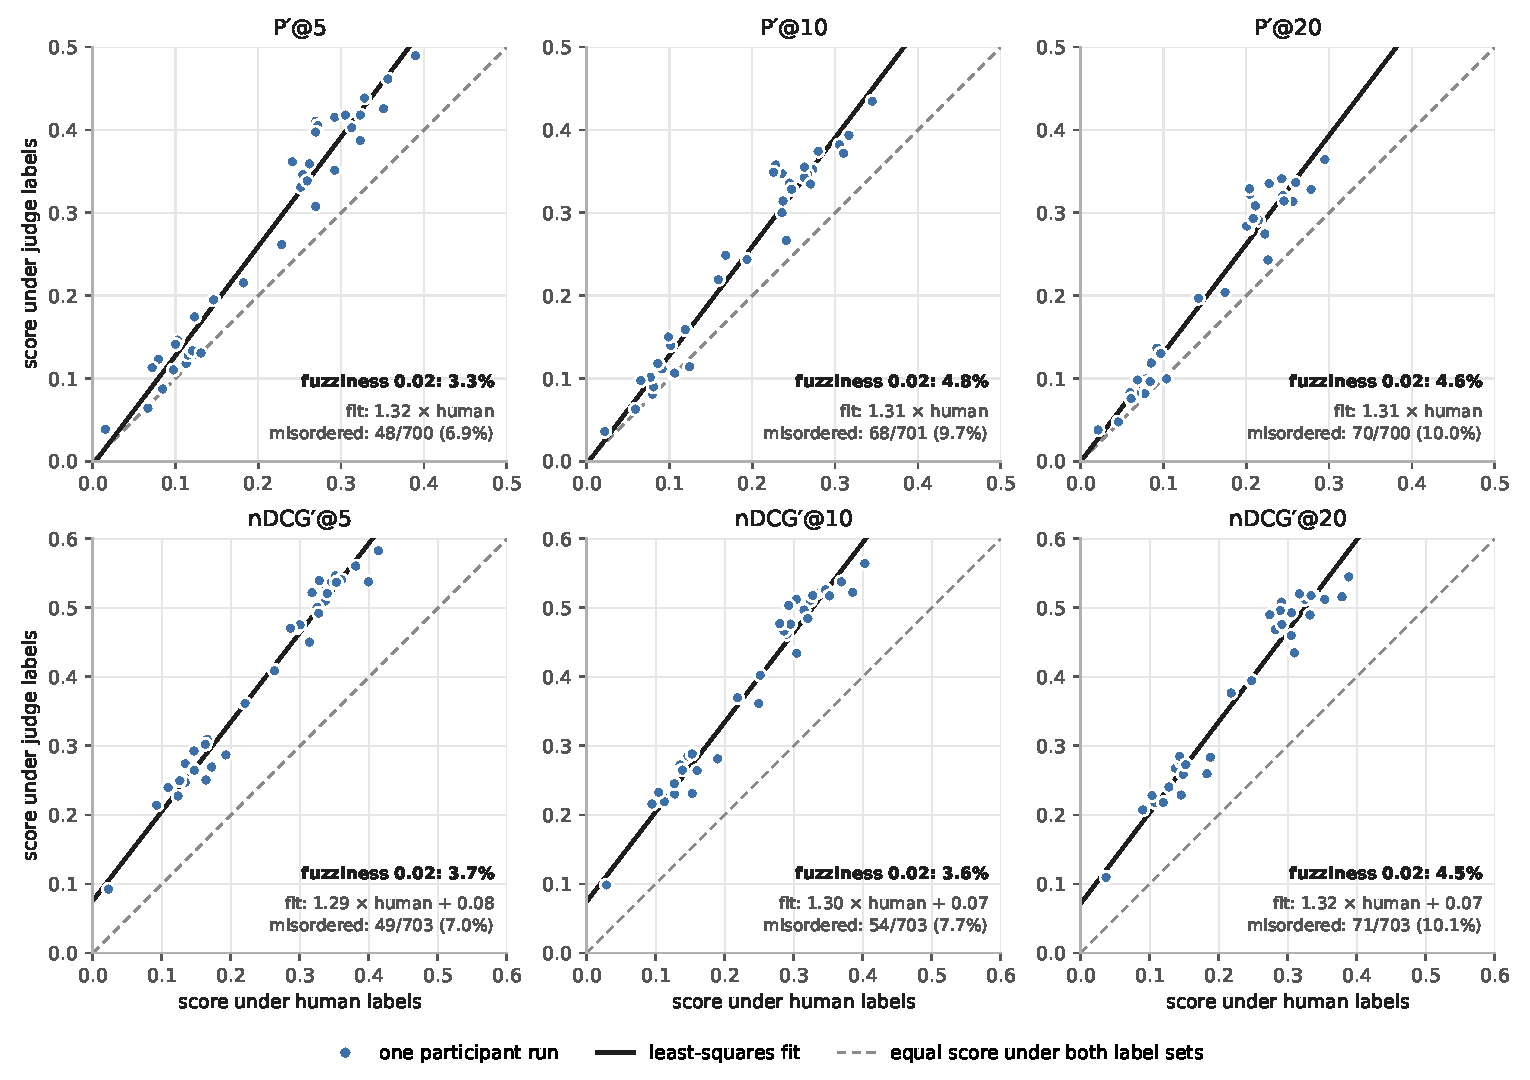
\includegraphics[width=\textwidth]{images/judge_calibration_r4.pdf}
\caption[Calibration of the relevance judge]{Calibration of the LLM relevance judge on ARQMath-3. Each point is one of
the 38 official participant runs, scored over its own top 20 answers on the 78 topics
of Section~\ref{sec:met-collection}: once under the assessors' labels (horizontal
axis) and once under the judge's (vertical axis). Top row: P$'$@$k$, precision at
$k$. Bottom row: nDCG$'$@$k$, normalised discounted cumulative gain at $k$. Solid
line: least-squares fit. Dashed line: equal score under both label sets.
\emph{Misordered}: pairs of runs that the two label sets place in opposite order, out
of all 703 pairs. For P$'$ the count is out of 700 or 701, because a few pairs of runs
receive exactly the same P$'$ under the judge's labels and cannot be ordered at all.
\emph{Fuzziness 0.02}: the share of pairs misordered when only pairs whose scores
under the judge's labels differ by more than 0.02 are counted, the only pairs later
chapters order.}
\label{fig:met-judge-calibration}
\end{figure}

In every panel the points lie close to a straight line ($R^2$ between 0.95 and 0.97).
The slope is between 1.29 and 1.32 for all six measures. The intercept is effectively
zero for P$'$ and 0.07 to 0.08 for nDCG$'$. The judge's scores are the assessors'
scores stretched: a participant run the assessors credit with 0.20 nDCG$'$@10 is
credited with about 0.33 under the judge's labels. A stretch of this kind cannot
reorder anything on its own, because multiplying two scores by the same positive
number and adding the same constant keeps the larger one larger. Only the scatter
around the line can reorder systems, and that is what the error rate measures.

The error rate is the share of pairs of participant runs that the two label sets
order differently. Taken over all 703 pairs, nDCG$'$@10 orders 54 of them
differently, or 7.7\%. That is close to the one pair in thirteen that the 2022 $\tau$
implied, although the two are computed differently. Across the six measures the rate
lies between 6.9\% and 10.1\%.

A fuzziness value treats pairs closer than a threshold as tied rather than ordered.
Those are the pairs the judge is most likely to get wrong, so raising the threshold
lowers the error rate among the pairs that remain, at the price of ordering fewer of
them. The threshold is applied to the difference in judge-label scores, since that is
the only difference a later chapter can observe.

At 0.02 the error rate falls below 5\% for every measure and cutoff: 3.3\%, 4.8\% and
4.6\% for P$'$ at 5, 10 and 20, and 3.7\%, 3.6\% and 4.5\% for nDCG$'$. At
nDCG$'$@10, 603 of the 703 pairs differ by more than 0.02 under the judge's labels;
the remaining 100 are treated as ties. In 581 of the 603, the judge's labels and the
assessors' labels agree on which run is better. In 22, or 3.6\%, they disagree. One
measure, nDCG$'$@5, would already fall below 5\% at 0.01. A single threshold for all
six is simpler to apply, and the measure every verdict reads, nDCG$'$@10, needs 0.02
in any case. For comparison, UMBRELA's authors report that their judge could not tell
apart systems closer than about 0.065 nDCG@20~\cite{upadhyay2025umbrela}. That figure
belongs to a different judge, collection and procedure, and is not used here.

This fixes the rule the retrieval and generation chapters follow. Two
systems scored against the same judge labels are ordered only when their scores,
reported to three decimals, differ by more than 0.02 on the measure and cutoff in
question. A difference of 0.02 or less is reported as indistinguishable. Above the
threshold the order is still not certain: it is wrong for fewer than one pair in
twenty, not for none. The scores themselves stay on the judge's inflated scale: a
system scoring 0.50 under the judge's labels is ahead of one scoring 0.47, but
neither number says what the assessors would have given.

The rule assumes that two systems being compared are scored against the same judge
labels. Which answers those labels cover is not settled here, because it depends on
what this thesis's systems retrieve; Section~\ref{sec:met-evaluation-protocol} builds
that set of labels from their rankings.

% --- (§4.5 Notation and reporting conventions -- REMOVED 2026-09-20) ------------
% Removed at Abram's request; the stub is parked as _sec45_notation.RETIRED.tex (not input).
% May return if required -- manifest §15 O-14.
